

% This is based on the LLNCS.DEM the demonstration file of
% the LaTeX macro package from Springer-Verlag
% for Lecture Notes in Computer Science,
% version 2.4 for LaTeX2e as of 16. April 2010
%
% See http://www.springer.com/computer/lncs/lncs+authors?SGWID=0-40209-0-0-0
% for the full guidelines.
%
\documentclass{llncs}
\usepackage[utf8]{inputenc}
\usepackage[ngerman]{babel}
\usepackage{graphicx}
\begin{document}
\title{HTTP und HTTP/2}
\author{Michael Hochleitner}
\institute{Ludwig-Maximilians-Universit\"at M\"unchen}

\maketitle 
\begin{center}
Bachelorseminar ``Web Technologies'' \\
Wintersemester 2017/18
\end{center}

\begin{abstract}
HTTP ist ein Netzwerkprotokoll, das benutzt wird um Datenpakete zwischen Rechnern in Rechnernetzen auszutauschen. Die erste Version von HTTP wurde 1990 entwickelt. Seitdem wurde das Protokoll in mehreren Protokollversionen erweitert. Die Schwerpunkte bei den Erweiterungen des Protokolls sind Flexibilität und Performanz. Flexibilität bedeutet, dass das Protokoll erweitert werden kann. Es können neue Anfragemethoden, Errorcodes und Header hinzugefügt werden. HTTP baut auf einem Transportprotokoll auf. Verbesserungen in der Performanz erreicht man durch effiziente Nutzung des Transportprotokolls. Das wird in HTTP/2 durch Multiplexing umgesetzt. Die prominenteste Anwendung, die HTTP nutzt, ist das World Wide Web.
\keywords{Protokoll, Rechnernetze, Internet, World Wide Web, Hypertext, HTTP, HTTP/2}
\end{abstract}

\section{Einleitung}

Der Informatiker Tim Berners-Lee arbeitete in den 90er Jahren in der Forschungseinrichtung CERN in Genf. Dort arbeiteten viele Leute, die verschiedene Computer und verschiedene Textverarbeitungsprogramme benutzten, um ihre Ergebnisse zu dokumentieren. Der Austausch von digitalen Dokumenten war schwierig. Deshalb entwickelte er ein Dokumentationssystem. \begin{quote}What I was looking for fell under the general category of documentation systems-software that allows documents to be stored and later retrieved. \cite{Berners-Lee1999} \end{quote}
Das Dokumentationssystem kombinierte die Technologien Internet, Hypertext und das Aufrufen von Prozeduren auf anderen Computern, genannt RPC (Remote Procedure Call). Es wurde bekannt unter dem Namen World Wide Web.\newline Die Architektur des World Wide Web ist Client-Server. Der Client sollte ein Programm sein, mit dem man Hypertextseiten erstellen, durchblättern und editieren kann.\cite{Berners-Lee1999} Der Server sollte ein Programm sein, das die Hypertextseiten hält und den Benutzern des World Wide Web Zugriff darauf erlaubt.\cite{Berners-Lee1999} 
Durch das gemeinsame Dateiformat HTML (Hypertext Markup Language), die Verbindung von Computern über das Internet und das Abspeichern der HTML-Dateien auf einem Server wurde es möglich im World Wide Web auf digitale Dokumente zuzugreifen, die nicht dauerhaft auf dem Computer gepeichert sein müssen, auf dem man sie liest. Somit konnte man von Computern mit verschiedenen Betriebssystemen auf einen gemeinsamen Speicherort für Dokumente zugreifen.\newline Um Dateien auf einem Server für andere Computer zur Verfügung zu stellen, versendet man die Dateien in Datenpaketen. Dafür benötigt man ein Protokoll. Das Protokoll des World Wide Web ist HTTP, das Hypertext Transfer Protocol.
\section{HTTP Grundlagen}
HTTP wurde entwickelt, um das Internet und HTML kompatibel zu machen. HTTP gibt es in vier Versionen. Die Versionsnummern sind 0.9, 1.0 1.1 und 2. Definiert wird HTTP in Requests for Comments, die von der Internet Engineering Task Force (IETF) und der Internet Society (ISOC) herausgegeben werden.

Die Versionsnummer 0.9 ist eine Versionsnummer, die im Nachhinein dem Prototypen von HTTP verliehen wurde. 1.0 ist die erste Versionsnummer, die in einem RFC veröffentlich wurde. Der RFC 1945 beschreibt HTTP 1.0, der RFC 2616 beschreibt HTTP 1.1 und der RFC 7540 beschreibt HTTP 2.0.
Die Version wurde 1.0 von den Autoren nicht als offizieller Standard gesehen, wie das folgende Zitat zeigt. \begin{quote} This Memo does not specify an Internet standard of any kind. \cite{Berners-Lee1996} \end{quote} Erst HTTP 1.1 bezeichnen die Autoren des RFCs als \begin{quote}[...] internet standards track protocol for the internet community. \cite{Fielding1999} \end{quote} HTTP 0.9 ist ein Protokoll mit dem man Datenpakete über eine TCP Verbindung verschicken kann. Das Protokoll definiert welche Form die Datenpakete haben müssen. Das Protokoll unterscheidet zwei Arten von Datenpaketen: Anfragen und Antworten. Anfragen sind dazu da, um Dateien anzufragen. Sie werden vom Client an den Server geschickt. Antworten enthalten bei einer erfolgreichen Anfrage die angefragte Datei. Um eine HTML Datei zu empfangen, muss ein Client über die TCP-Verbindung eine Anfrage schicken. In der Anfrage wird die Datei, die übertragen werden soll spezifiziert. Es folgt ein Beispiel für eine Anfrage.
\begin{verbatim}
GET /index.html
\end{verbatim}
Die Methode in dieser Anfrage ist GET. Sie bedeutet, dass eine Datei vom Server zum Client übertragen werden soll. Der Server, die IP-Adresse und der Port müssen in HTTP-Anfragen nicht spezifiziert werden. Das ist Aufgabe der unterliegenden Protokolle IP und TCP. Die GET-Methode bekommt als Parameter eine URI. Die URI ist die Adresse der Datei.\newline
Wenn eine Anfrage bei einem Server ankommt, muss er entscheiden, ob er die angeforderte HTML-Datei verschicken kann. Wenn er das kann ist die Antwort in der Protokollversion 0.9 die angefragte HTML-Datei. Der RFC 2616 bezeichnet das als ``raw data transfer''.\newline Aufgrund des Anfrage-Antwort-Mechanismus, den HTTP nutzt, wird es der Gruppe der Request-Response-Protokolle zugeordnet. Die Codierung für die Protokollversionen 0.9, 1.0 und 1.1 ist ASCII. Das ist so, weil die Devise bei der Entwicklung von HTTP 0.9 war möglichst wenig über die Computer, die über das Protokoll kommunizieren sollten anzunehmen: \begin{quote} The least common denominator we could assume among all different types of computers was that they all head some sort of keyboard input device, and they all could produce ASCII (plain text) characters. \cite{Berners-Lee1999} \end{quote} Die HTTP Version 0.9 eignet sich gut um den Request-Response-Charakter von HTTP anschaulich darzustellen, weil die Anfragen und Antworten sehr kompakt sind. Das ist bei den Versionen mit höheren Versionsnummern nicht so. Es folgt ein Beispiel für eine Antwort, die mit HTTP 0.9 konform ist.
\begin{verbatim}
<html>
<p> Das ist eine HTML-Seite.<\p>
</html>
\end{verbatim}
\section{Methoden}
Der wichtigste Bestandteil eines HTTP-Pakets ist die Methode. Ein Datenaustausch zwischen Client und Server geht normalerweise vom Client aus. Der schickt ein Paket, das eine Methode enthält. Sie sagt dem Server was der Client will. Weiter oben wurde die GET-Methode beschrieben. Die beiden wichtigsten Methoden sind GET und HEAD. \begin{quote} The methods GET and HEAD MUST be supported by all general-purpose servers.\cite{Fielding1999} \end{quote}
Außerdem gibt es OPTIONS, POST, PUT, DELETE, TRACE und CONNECT. Mit der HEAD Methode kann Metadaten über eine Ressource abfragen, ohne sie zu übertragen. Die Antwort auf einen HEAD-Request enthält Headerfelder ohne den zugehörigen Entity-Body.  PUT bedeutet, dass der Paketinhalt unter der angegebenen URI auf dem Server gespeichert werden soll. POST gibt eine übergeordnete URI an, unter der der Paketinhalt der Anfrage gespeichert werden soll. So wie man auf einem Dateisystem eine Datei in einem Ordner speichert. Die URI des Paketinhalts, der auf dem Server gespeichert wurde, wird in einer Antwort vom Server zurückgeschickt. Das ist eine Anwendungsmöglichkeit eines POST-Requests. Man kann mit einem POST-Request auch Daten aus einem Formular an einen Prozess auf dem Server leiten, der die Daten weiterverarbeitet.
Die Gemeinsamkeit aller POST-Anfragen ist, das der Paketinhalt vom Server weiterverarbeitet wird. Die Definitionen der anderen Methoden kann man im RFC 2616 nachlesen.
\section{Header}
Während man mit dem HTTP-Protokoll in der Version 0.9 nur HTML-Dateien verschicken konnte, ist es ab der Protokollversion 1.0 auch möglich andere Dateitypen zu verschicken. Das Protokoll ermöglicht es, dass ein Paket die Information enthält, welchen Dateityp das Paket verpackt. Diese Metadaten sind im Header. Der Header eines Pakets besteht aus einem oder mehreren Headerfeldern. Die Aufteilung in Metadaten und Pakethinhalt führt dazu, dass ein Antwort-Paket nach Protokollversion 1.0 eine andere Struktur hat als ein Paket nach Protokollversion 0.9. Während in Version 0.9 nur eine HTML-Datei enthalten ist, kann ein Antwort-Paket ab Version 1.0 auch einen Header enthalten, der den Inhalt des Paketes beschreibt. Die Kombination von Metadaten und Inhalt heißt Entity. Den Inhalt bezeichnet man auch als Payload oder Entity-Body.
\begin{quote}   entity \linebreak

       A particular representation or rendition of a data resource, or
       reply from a service resource, that may be enclosed within a
       request or response message. An entity consists of
       metainformation in the form of entity headers and content in the
       form of an entity body. \cite{Berners-Lee1996} \end{quote} \
   Es folgt ein Beispiel für ein Headerfeld.
\begin{verbatim}
Content-Type: text/html; charset=UTF-8
\end{verbatim}
Der hier gezeigte Header ist dafür da, um den Datentyp eines Paketinhalts anzuzeigen. Wie man oben sieht, sind Header Paare aus Name und Wert, die durch einen Doppelpunkt getrennt sind. [Hier kann ich noch etwas über MIME schreiben.] \linebreak Es gibt verschiedene Arten von Headern. Sie erfüllen unterschiedliche Funktionen. Sie sind in drei Gruppen eingeteilt: Allgemeine Headerfelder, Anfrage-Headerfelder, Antwort-Headerfelder und Entity-Headerfelder.\cite{Fielding1999} Entity-Headerfelder beschreiben den Entity-Body. Das Connection-Headerfeld ist ein Entity-Headerfeld. Anfrage Headerfelder dürfen nur in Anfragen benutzt werden, Antwort-Headerfelder nur in Antworten.  Allgemeine Headerfelder sind in Anfragen und Antworten erlaubt. Ein Beispiel für ein allgemeines Headerfeld ist das Connection-Headerfeld: 

\begin{verbatim}
Connection: close
\end{verbatim}
Wenn dieses Headerfeld in einer Anfrage mitgeschickt wird, sagt es aus, dass die Verbindung nach Bearbeitung der Anfrage geschlossen werden kann. \linebreak
Der wichtigste Anfrage Header ist Host. \begin{quote} The Host request-header field (section 14.23) MUST accompany all
   HTTP/1.1 requests. \cite{Fielding1999} \end{quote} Er ist dafür da, dass blablabla.
\section{Statuscodes}
Die Antworten nach Protokollversion 0.9 die oben als Raw Data Transfer bezeichnet wurden, nennt der RFC 1945 Simple-Response. Die unterscheidet er von einer Full-Response. Das Unterscheidungsmerkmal ist eine Status-Line. Die Status-Line enthält die Protokollversion, einen Statuscode und eine textuelle Beschreibung des Statuscodes. Es folgt ein Beispiel.
\begin{verbatim}
HTTP/1.0 302 Found
\end{verbatim}
Statuscodes beschreiben, ob der Server die Anfrage verstanden hat und ob er die gewünschte Aktion ausgeführt hat. Ein Statuscode ist eine Zahl zwischen 99 und 600. Alle Statuscodes mit der selben Hunderterstelle bilden eine Klasse.\newline
Die Klasse 1xx heißt Informational. Sie sagt aus, dass das die Anfrage empfangen wurde und noch in Bearbeitung ist.\newline
Die Klasse 2xx heißt Success. Sie sagt aus, dass die Anfrage empfangen, verstanden und akzeptiert wurde.\newline
Die Klasse 3xx heißt Redirection. Sie sagt aus, dass weitere Aktionen nötig sind, um die Anfrage vollständig zu bearbeiten.\newline
Die Klasse 4xx heißt Client Error. Sie sagt aus, dass die Anfrage syntaktisch nicht korrekt ist oder die gewünschte Aktion nicht ausgeführt werden kann.\newline
Die Klasse 5xx heißt Server Error. Sie sagt aus, dass der Server eine in einer validen Anfrage gewünschte Aktion nicht durchführen konnte. \newline
Diese Beschreibung sind Übersetzungen aus \cite{Fielding1999}. \newline
Der Statuscode 302 aus der Klasse Redirection sagt aus, dass die angefragte Ressource temporär unter einem anderen URI erreichbar ist. Diese temporäre URI wird dem Client in der Antwort im Location-Headerfeld mitgeteilt. Der Client muss die neue URI anfragen, damit sein ursprünglicher Request vollständig bearbeitet wird. Das ist die weitere Aktion, die charakteristisch für Statuscodes der Klasse 3xx ist. 
   
\section{Performanz und HTTP/2}
Zur Zeit der Protokollversion 0.9 bestanden Internetseiten nur aus Text, der als einzelne HTML-Datei versendet werden konnte. Im Laufe der Zeit stieg die Anzahl der Requests, die ein Browser sendet, um eine Seite im World Wide Web anzuzeigen.Man verschickt ca. 200 Anfragen wenn man die Seite\linebreak https://de.yahoo.com/ aufruft. Siehe Abbildung 1.\newline Mit der Anzahl der Anfragen steigt auch die Anzahl der Dateien, die in Antworten zurückgesendet werden. Dementsprechend wurde HTTP im Laufe der Zeit angepasst. Den Benutzern des des World Wide Web sollen Internetseiten möglichst schnell angezeigt werden.
HTTP-Pakete werden über eine TCP-Verbindung verschickt. Eine effiziente Nutzung der TCP-Verbindung ermöglicht es viele Datenpakete in kurzer Zeit zu übertragen und eine Internetseite schnell aufzubauen.\newline

\begin{figure}
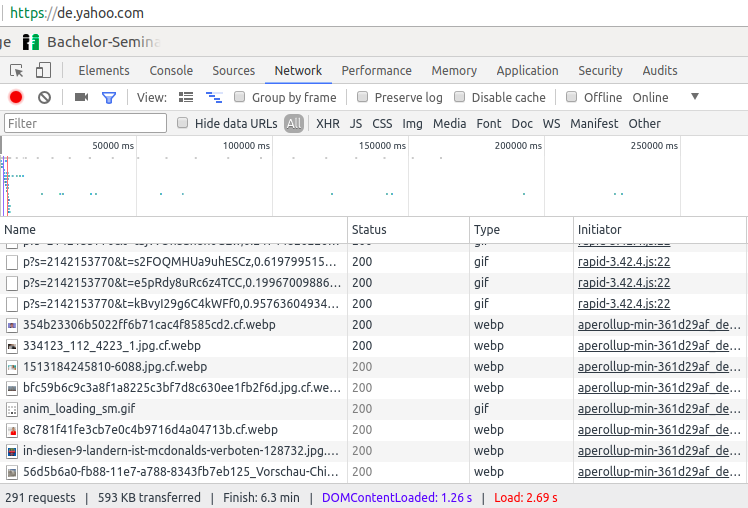
\includegraphics[width=\columnwidth]{yahooRequests}
\caption{Aufrufen von https://de.yahoo.com am 19.02.2018 im Browser Chromium. Links unten sieht man die Anzahl der Anfragen.}
\end{figure}
In der Protokollversion 0.9 gab es pro Anfrage-Antwort-Paar nur eine TCP-Verbindung. Die Verbindung wird für eine Anfrage geöffnet und nach der Über-tragung der Antwort geschlossen. Das Öffnen und Schließen einer TCP-Verbindung erzeugt einen Overhead. Um ihn zu entfernen wurden in HTTP/1.1 persistente Verbindungen eingeführt. Auf einer persistenten Verbindung kann man eine zweite Anfrage versenden ohne die Antwort auf die erste Anfrage abzuwarten. Das nennt der RFC 2616 Pipelining. Pipelining ist in Abbildung 2 dargestellt.

Wenn mehrere Anfragen in einer Pipeline auf einer TCP-Verbindung stehen, werden die Anfragen nacheinander abgearbeitet. Eine Anfrage deren Bearbeitung lange dauert kann die Bearbeitung der Anfragen dahinter verzögern. Dieses Phänomen heißt Head-of-line-Blocking oder HOL-Blocking. Wenn auf einer TCP-Verbindung HOL-Blocking auftritt kann eine neue Verbindung zum Server geöffnet werden, um neue Requests zu verschicken. Auf der neuen Verbindung kann wieder HOL-Blocking auftreten. Da die Anzahl der TCP-Verbindungen zwischen Client und Server begrenzt ist, können alle Verbindungen durch HOL-Blocking blockiert werden. HOL-Blocking ist ein Hindernis, dass die Ladezeit einer Website erheblich beeinträchtigt.

Um diesem Problem zu begegnen, wurde in HTTP/2 Multiplexing eingeführt.
\begin{figure}
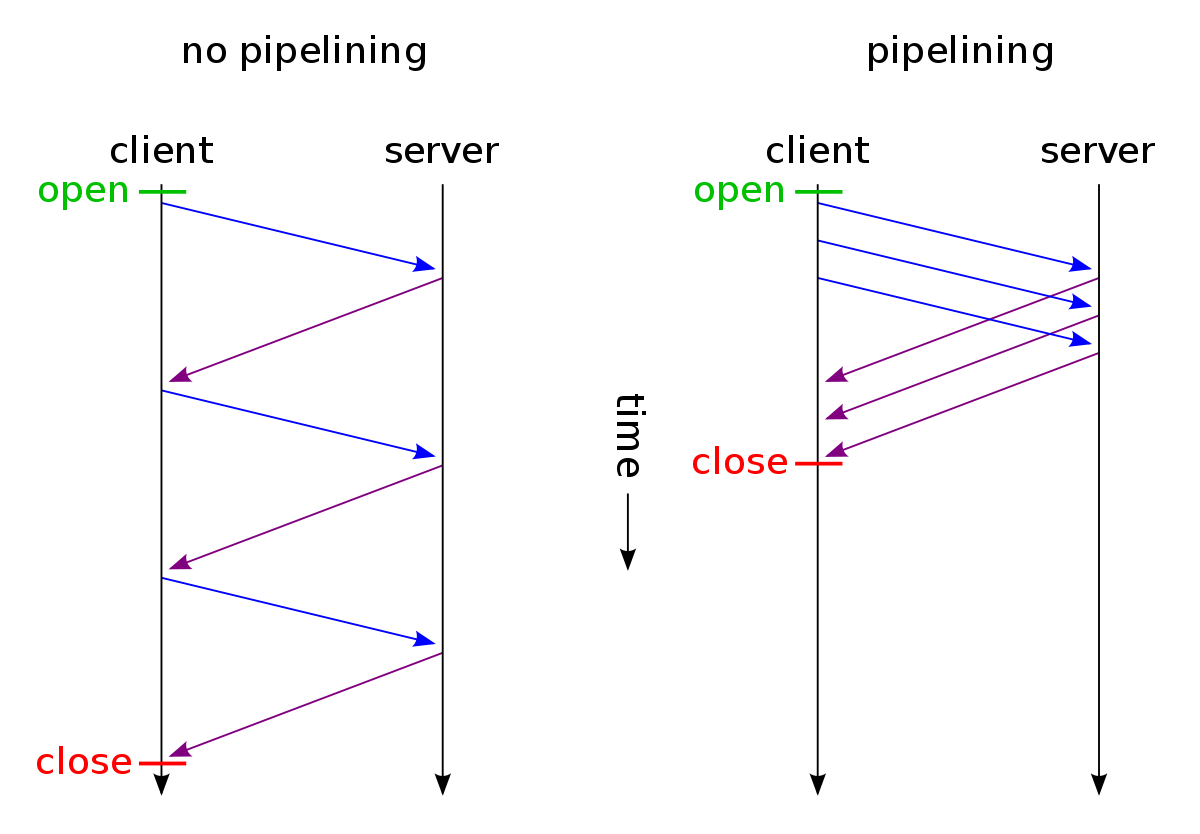
\includegraphics[width=\columnwidth]{1200px-HTTP_pipelining2}
\caption{Pipelining erlaubt es eine Anfrage zu senden ohne auf die Antwort der vorhergehenden Anfrage zu warten.}
\end{figure}


In HTTP/2 gibt es Multiplexing.\cite{Belshe2015}

\section{Zusammenfassung}
HTTP ist ein Request-Response-Protokoll, das zum Datenaustausch zwischen Computern über ein Rechnernetz genutzt wird. Es wurde ursprünglich für ein Dokumentationssystem entwickelt, das den Austausch digitaler Dokument zwischen Rechnern mit verschiedenen Betriebssystemen ermöglichen sollte. Dieses Dokumentationssystem hat sich zum World Wide Web entwickelt. 
HTTP kommt zum Einsatz wenn ein Browser eine Internetseite von einem Server anfragt.\newline Ein HTTP-Paket enthält eine Methode, Metadaten und einen Payload. Die Methode drückt die Handlung aus, die der Client vom Server erwartet. Metadaten in HTTP-Paketen sind Header und Statuscodes. Der Payload ist eine Datei, die der Client zum Server übertragen will oder vom Server anfragt. \newline
HTTP baut auf dem Transportprotokoll TCP auf.
Die Verwendung von TCP-Verbindungen hat großen Einfluss darauf wie schnell eine Internetseite angezeigt werden kann. Die Verwendung der TCP-Verbindungen hat sich vom Öffnen und Schließen einer Verbindung für jede HTTP-Anfrage über persistente Verbindungen mit Pipelining zum Multiplexing entwickelt. \newline
HOL-Blocking auf Ebene von HTTP-Paketen wurde in HTTP/2 mit Multiplexing gelöst.
 Auf der Ebene von TCP-Paketen gibt es auch HOL-Blocking. Dafür entwickelt Google ein alternatives Protokoll unter dem Namen QUIC. 
\bibliographystyle{acm}
\bibliography{literature}


\end{document}

              
 

